\documentclass[11pt]{article}
\usepackage{natbib,mybigpackage}
\usepackage{algorithm}
%\usepackage{program}
%\usepackage{algpseudocode}
\usepackage{algorithmic}
\usepackage{listings}


\def\xbf{\mathbf{x}}
\def\zbf{\mathbf{z}}
\def\xibf{\mathbf{\xi}}
\title{Documentation: Assignment 5}
\author{Abhinav Gupta\
 150123001}
\begin{document}
\titlepage
\newpage

\begin{enumerate}
\item[Q 1] Generate 1000 standard normal variates using standard Double-exponential distribution by acceptance-rejection method. Calculate the necessary constant c, where \[f(x)/g(x)<=c\]\[f(x) and g(x) \]are the pdfs of standard normal and standard Double-exponential distribution respectively. Calculate the the
oretical and simulated acceptance probability. How do you justify your generated random numbers are correct ?
Provide as many verification as you can.
\end{enumerate}

\noindent{Code: R}

\begin{lstlisting}
count<-0
gInv<-function(u){
	if(u<1/2){
		return (log(2*u))
	}
	else{
		return (-1*log(2*(1-u)))
	}
}
c=sqrt(2*exp(1)/pi)
f<-function(x){
	return (sqrt(1/(2*pi))*exp(-1*x*x/2))
}
g<-function(x){
	return ((1/2)*exp(-1*abs(x)))
}
vector<-c()
total<-0
while(1){
u1<-runif(1)
u2<-runif(1)
x<-gInv(u1)
if(u2<=(f(x)/(c*g(x)))) {
cat("Sample Values are: ",x)
cat("\n")
count<-count+1
vector[count]<-x
}
total<-total+1
if(count==1000)
break
}
cat("\nSimulated Acceptance: ",count/total)
cat("\nTheoretical Acceptance: ",1/c)
cat("\nMean: ",mean(vector))
cat("\nVariance: ",var(vector))
png("question1.png")
hist(vector, breaks=50 , col="light cyan",plot=TRUE)
cat("\n")
\end{lstlisting}

\noindent{\textbf{Output}:}

Simulated Acceptance:  0.7745933\

Theoretical Acceptance:  0.7601735\

Mean:  0.04431985\

Variance:  0.9399264\

\noindent{\textbf{Observation}:}
\begin{equation}
g(x)=1/2*e^{(-|x|)}
\end{equation}
\begin{equation}
f(x)=\sqrt{1/2\pi} *e^{(-x^2/2)}
\end{equation}
\begin{equation}
f(x)/g(x)=\sqrt{2/\pi}e^{(-x^2/2+|x|)}<=\sqrt{2e/\pi}=constant
\end{equation}
\begin{itemize}
	\item{Simulated acceptance probability: 0.7745933}
	\item{Theoretical acceptance probability: 0.7601735}
	\item{\textbf{Justification of why my random numbers are correct}: }
	As my mean and variance are closer to the standard normal function's respective attributes and also graph is similar to it. So my output is near to correct distribution. 

	\textbf{Mean: 0.04431985}\

	\textbf{Variance: 0.9399264}\

	\textbf{Graph: }\


\end{itemize}
  \begin{figure}[H]
  \centering
 \subfloat[using R]{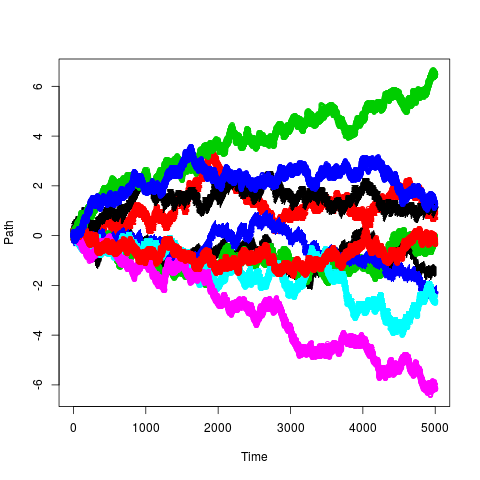
\includegraphics[width=1\textwidth]{question1.png}}\\
\end{figure}

%----------------------------------------------------------------------------------------------------------
\begin{enumerate}
\item[Q 2] Do the same exercise for generating random numbers from half-standard normal distribution using exponential distribution with mean 1 by acceptance-rejection method.
\end{enumerate}

\noindent{Code: R}
\begin{lstlisting}
count<-0
gInv<-function(u){
	return(-1*log(1-u))
}
c=sqrt(2*exp(1)/pi)
f<-function(x){
	return (2*sqrt(1/(2*pi))*exp(-1*x*x/2))
}
g<-function(x){
	return (exp(-1*x))
}
vector<-c()
total<-0
while(1){
u1<-runif(1)
u2<-runif(1)
x<-gInv(u1)
if(u2<=(f(x)/(c*g(x)))) {
cat("Sample Values are: ",x)
cat("\n")
count<-count+1
vector[count]<-x
}
total<-total+1
if(count==10000)
break
}
cat("\nSimulated Acceptance: ",count/total)
cat("\nTheoretical Acceptance: ",1/c)
cat("\nMean: ",mean(vector))
cat("\nVariance: ",var(vector))
png("question2.png")
hist(vector, breaks=50 , col="light cyan",plot=TRUE)
cat("\n")
\end{lstlisting}

\noindent{\textbf{Output}:}

Simulated Acceptance:  0.7628347\

Theoretical Acceptance:  0.7601735\

Mean:  0.8043221\

Variance:  0.367382\


\noindent{\textbf{Observation}:}
\begin{equation}
g(x)=e^{(-x)}
\end{equation}
\begin{equation}
f(x)=2\sqrt{1/2\pi} *e^{(-x^2/2)}
\end{equation}
\begin{equation}
f(x)/g(x)<=\sqrt{2e/\pi}=constant
\end{equation}
\begin{itemize}
	\item{Simulated acceptance probability: 0.7628347}
	\item{Theoretical acceptance probability: 0.7601735}
	\item{\textbf{Justification of why my random numbers are correct}: }
	As my mean and variance are closer to the standard half normal function's respective attributes and also graph is similar to it. So my output is near to correct distribution. 

	\textbf{Mean: 0.8043221}\

	\textbf{Variance: 0.367382}\

	\textbf{Graph: }\


\end{itemize}
\begin{figure}[H]
  \centering
 \subfloat[Using R]{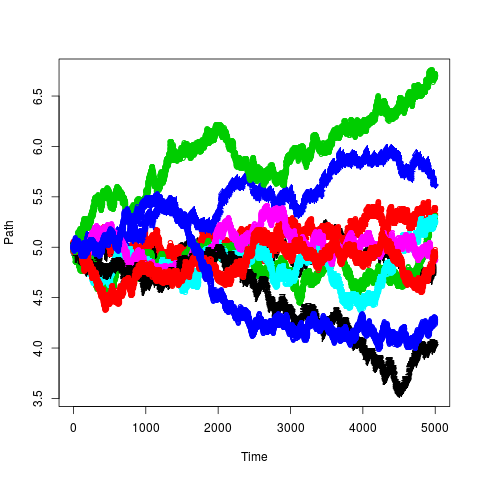
\includegraphics[width=1\textwidth]{question2.png}}\\
\end{figure}

%---------------------------------------------------------------------------
\begin{enumerate}
\item[Q 3] Consider the following discrete distribution.

a) Generate 10 random numbers from the above probability mas
s function using usual
procedure (inverse transform) of generating random number
from discrete distribution
defined on finite number of points. Calculate mean and varianc
e of the generated
numbers.\

b) Generate 10 random numbers from the same probability mass
function by acceptance-
rejection principle. Calculate mean and variance of the gen
erated numbers
\end{enumerate}

\noindent{Code for part "A": Inverse Transform}

\begin{lstlisting}
cdf<-c(0.05,0.30,0.75,0.90,1.0)
values<-c(1,2,3,4,5)
samples<-c()
count<-0
while(count!=10){
	u<-runif(1)
	for(i in 1:5){
		if(u<=cdf[i]){
			count<-count+1
			samples[count]=values[i]
			cat("\nSample Values are: ",samples[count])
			break
		}
	}
}
cat("\nMean: ",mean(samples))
cat("\nVariance: ",var(samples))
cat("\n")
\end{lstlisting}


\noindent{\textbf{Output of Inverse Transform generated from 10 values}:}

\textbf{Mean: 3.1}\

\textbf{Variance: 1.433333}\



\noindent{Code for part "B": Acceptance Rejection}

\begin{lstlisting}
pdf<-c(0.05,0.25,0.45,0.15,0.10)
values<-c(1,2,3,4,5)
samples<-c()
N<-5
count<-0
max<-0
gInv<-function(u){
	return(floor(N*u)+1)
}
for(i in 1:N){
	if(max<=(pdf[i]*N)) {
		max<-pdf[i]*N
	}
}
f<-function(x){
	return (pdf[x])
}
g<-function(){
	return (1/N)
}
while(1){
u1<-runif(1)
u2<-runif(1)
x<-gInv(u1)
if(u2<=(f(x)/(max*g()))) {
cat("Sample Values are: ",x)
cat("\n")
count<-count+1
samples[count]<-x
}
if(count==10)
break
}
cat("\nMean: ",mean(samples))
cat("\nVariance: ",var(samples))
cat("\n")
\end{lstlisting}

\noindent{\textbf{Output of Acceptance Rejection generated from 10 values}:}

\textbf{Mean: 3.2}\

\textbf{Variance: 0.8444444}\


\end{document}
